\documentclass[
%% TIKZ_CLASSOPTION %%
tikz
]{standalone}
\usepackage{amsmath}
\usetikzlibrary{matrix}
%% EXTRA_TIKZ_PREAMBLE_CODE %%
\begin{document}
%% TIKZ_CODE %%
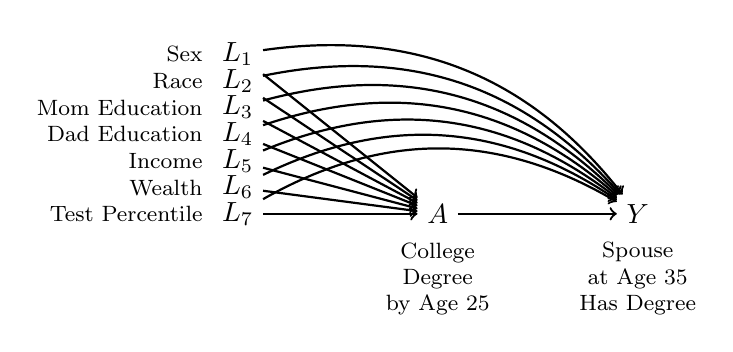
\begin{tikzpicture}[x = 1in, y = .4in]
\node (a) at (0,0) {$A$};
\node (y) at (1,0) {$Y$};
\node (l1) at (-1,2) {$L_1$};
\node (l2) at (-1,1.66) {$L_2$};
\node (l3) at (-1,1.33) {$L_3$};
\node (l4) at (-1,1) {$L_4$};
\node (l5) at (-1,.66) {$L_5$};
\node (l6) at (-1,.33) {$L_6$};
\node (l7) at (-1,0) {$L_7$};
\draw[->, thick] (l1) -- (a);
\draw[->, thick] (l2) -- (a);
\draw[->, thick] (l3) -- (a);
\draw[->, thick] (l4) -- (a);
\draw[->, thick] (l5) -- (a);
\draw[->, thick] (l6) -- (a);
\draw[->, thick] (l7) -- (a);
\draw[->, thick] (a) -- (y);
\draw[->, thick] (l1) to[bend left] (y);
\draw[->, thick] (l2) to[bend left] (y);
\draw[->, thick] (l3) to[bend left] (y);
\draw[->, thick] (l4) to[bend left] (y);
\draw[->, thick] (l5) to[bend left] (y);
\draw[->, thick] (l6) to[bend left] (y);
\draw[->, thick] (l7) to[bend left] (y);
\node[anchor = north, align = center, font = \footnotesize] at (a.south) {College\\Degree\\by Age 25};
\node[anchor = north, align = center, font = \footnotesize] at (y.south) {Spouse\\at Age 35\\Has Degree};
\node[anchor = east, align = center, font = \footnotesize] at (l1.west) {Sex};
\node[anchor = east, align = center, font = \footnotesize] at (l2.west) {Race};
\node[anchor = east, align = center, font = \footnotesize] at (l3.west) {Mom Education};
\node[anchor = east, align = center, font = \footnotesize] at (l4.west) {Dad Education};
\node[anchor = east, align = center, font = \footnotesize] at (l5.west) {Income};
\node[anchor = east, align = center, font = \footnotesize] at (l6.west) {Wealth};
\node[anchor = east, align = center, font = \footnotesize] at (l7.west) {Test Percentile};
\end{tikzpicture}
\end{document}
